\documentclass[paper = letter, fontsize = 11pt]{scrartcl}
\usepackage[T1]{fontenc}
\usepackage[english]{babel}
\usepackage{geometry}
\geometry{margin = 1in}
\usepackage{sectsty}
\usepackage{graphicx}
\usepackage{amsmath}
\allsectionsfont{\centering \normalfont\scshape}
\usepackage{fancyhdr}
\pagestyle{fancyplain}
\fancyhead{}
\fancyfoot[C]{\thepage}
\renewcommand{\headrulewidth}{0pt}
\renewcommand{\footrulewidth}{0pt}
\setlength{\headheight}{13.6pt}
\setlength\parindent{12pt}
%	TITLE
\newcommand{\horrule}[1]{\rule{\linewidth}{#1}}
\title{	
\normalfont \normalsize 
\textsc{Delaware Valley Regional Planning Commission} \\ [25pt]
\horrule{0.5pt} \\[0.4cm]
\huge Employment Data Evaluation \\
\horrule{2pt} \\[0.5cm]
}
\author{\normalsize Addison Larson}
\date{\normalsize\today}
%	BODY
\begin{document}
\maketitle
\section{Overview}
This paper evaluates differences in the 2013 vintage of two purchased employment data sources---the National Establishment Time-Series (NETS) and InfoGroup---for Conshohocken, Montgomery County, PA. Specifically, these two datasets are evaluated based on summations of employment over census blocks, block groups, and tracts; the overall composition of establishments by number employed; establishment-level differences in employment; differences in large employers; and overall data quality. See Table 1, \textit{General Properties of NETS and InfoGroup Data for Conshohocken}, for a brief overview of the two datasets.\par
The Delaware Valley Regional Planning Commission (DVRPC) purchases NETS data when it becomes available. This occurred most recently in 2013. However, NETS data requires extensive manual cleanup for DVRPC's nine-county region. If InfoGroup data requires substantially less correction, then it may be worth the additional cost to purchase it instead of NETS. This study assumes NETS data is already clean and consistent.\par
There are critical differences between NETS and InfoGroup data sources, as well as between these sources and LEHD LEHD (Longitudinal Employer-Household Dynamics) data.
\begin{enumerate}
	\item \textbf{NETS} is a mystery.
	\item \textbf{InfoGroup} is also a mystery. Doesn't this have sole proprietors?
	\item \textbf{LEHD} is publicly-available employment and origin-destination data from the Census Bureau. It is synthesized from multiple imputation of tax and employment records and aggregated to the block level. Because of privacy concerns, noise is introduced in the data. Even though LEHD data is derived from tax records, it is likely geocoded using the Census Geocoder, which is less spatially accurate than other geocoding options \textbf{\textit{HALP! Is this true? Or is it that something like Google can better handle idiosyncracies in address quality?}}.
\end{enumerate}
\paragraph{Conflicting Signals.}
\begin{table}[h]
	\begin{center}
		\begin{tabular}{ r | c c }
			 & NETS & InfoGroup  \\
			\hline
			\hline
			Total Number of Establishments & 637 & 304 \\
			\hline 
			No. Establishments > 0 Employees & 631 & 286 \\
			\hline 
			No. Establishments > 50 Employees & 24 & 19 \\
			\hline
			Proposed Sample Size (90\% CI, MOE $\pm$ 5\%) & 143 & --- \\
			\hline  
		\end{tabular}
	\end{center}
	\caption{General Properties of NETS and InfoGroup Data for Conshohocken.}
\end{table}
\clearpage
\section{Summations of Employment Counts by Geographic Level}
When InfoGroup and NETS point-level employment data are aggregated to the block, block group, and census tract level, the counts differ greatly within each spatial unit. This section uses 2015 LEHD Workplace Area Characteristics as an employment comparison for NETS and InfoGroup.
\paragraph{Block-Level Differences.} Table 2, \textit{Differences in Employment, Block Level}, includes the counts by block and three additional columns: NETS x IG, NETS x LEHD, and IG x LEHD. A value of ``Yes'' in any of these columns indicates absolute percentage difference\footnote{The absolute percentage difference is calculated as: \[ \frac{\lvert v_{1} - v_{2} \rvert}{\frac{v_{1} + v_{2}}{2}} \times 100 \]} between the counts in the datasets in excess of 100\%. The results of the absolute percentage difference calculations indicate that InfoGroup and LEHD counts are the most similar at the block level, with 17 of 46 blocks differing over 100\% in job counts.
\paragraph{Block Group- and Tract-Level Differences.} It is suspicious that InfoGroup has 655 employees recorded for Block Group 420912041021 and Tract 42091204102, given that NETS and InfoGroup have nearly zero employees recorded for the same area. In addition, it is suspicious that LEHD has 180 employees recorded for Block Group 420912059062 and Tract 42091205906, when neither NETS nor InfoGroup have similar counts. The latter discrepancy may be attributable to the different source years of the data, since LEHD data comes from 2015. The discrepancies may also point to the need to manually correct both InfoGroup \textit{and} LEHD data.
\paragraph{Overall Count Differences.} In general, NETS has little in common with either InfoGroup or LEHD. LEHD has the fewest job counts overall, at 4,311. NETS has nearly 1,500 more jobs than LEHD for the neighborhood of Conshohocken---this hints that one of these datasets must be far off the mark.
\clearpage
\pagestyle{empty}
\begin{table}
	\begin{center}
		\begin{tabular}{ r | c c c c c c }
			Block GEOID & NETS & InfoGroup & LEHD & NETS x IG & NETS x LEHD & IG x LEHD\\
			\hline
			\hline
			420912041021003 & 0 & 655 & 16 & Yes & Yes & Yes\\
			\hline 
			420912042001006 & 72 & 0 & 0 & Yes & Yes & No\\
			\hline 
			420912042001008 & 430 & 1071 & 195 & No & No & Yes\\
			\hline 
			420912042001009 & 880 & 427 & 584 & No & No & No\\
			\hline 
			420912042001011 & 1056 & 551 & 105 & No & Yes & Yes\\
			\hline 
			420912042001012 & 858 & 24 & 34 & Yes & Yes & No\\
			\hline 
			420912042001014 & 33 & 34 & 118 & No & Yes & Yes\\
			\hline 
			420912042001015 & 1 & 0 & 0 & Yes & Yes & No\\
			\hline 
			420912042001016 & 41 & 44 & 34 & No & No & No\\
			\hline 
			420912042001018 & 110 & 24 & 23 & Yes & Yes & No\\
			\hline 
			420912042001019 & 2 & 0 & 1 & Yes & No & Yes\\
			\hline 
			420912042001021 & 60 & 57 & 106 & No & No & No\\
			\hline 
			420912042001022 & 44 & 44 & 9 & No & Yes & Yes\\
			\hline 
			420912042001034 & 63 & 176 & 0 & No & Yes & Yes\\
			\hline 
			420912042001035 & 93 & 493 & 542 & Yes & Yes & No\\
			\hline 
			420912042001037 & 4 & 5 & 1481 & No & Yes & Yes\\
			\hline 
			420912042001038 & 8 & 0 & 3 & Yes & No & Yes\\
			\hline 
			420912042001039 & 3 & 0 & 1 & Yes & No & Yes\\
			\hline 
			420912042001040 & 25 & 17 & 2 & No & Yes & Yes\\
			\hline 
			420912042001041 & 1 & 0 & 0 & Yes & Yes & No\\
			\hline 
			420912042001048 & 126 & 64 & 36 & No & Yes & No\\
			\hline 
			420912042001054 & 1 & 0 & 0 & Yes & Yes & No\\
			\hline 
			420912042001056 & 2 & 0 & 0 & Yes & Yes & No\\
			\hline 
			420912042002000 & 317 & 287 & 126 & No & No & No\\
			\hline 
			420912042002002 & 86 & 27 & 0 & Yes & Yes & Yes\\
			\hline 
			420912042002005 & 16 & 2 & 8 & Yes & No & Yes\\
			\hline 
			420912042002006 & 2 & 5 & 0 & No & Yes & Yes\\
			\hline 
			420912042002008 & 284 & 3 & 1 & Yes & Yes & No\\
			\hline 
			420912042002009 & 3 & 0 & 0 & Yes & Yes & No\\
			\hline 
			420912042002010 & 2 & 0 & 0 & Yes & Yes & No\\
			\hline 
			420912042002012 & 746 & 547 & 468 & No & No & No\\
			\hline 
			420912042002013 & 54 & 0 & 6 & Yes & Yes & Yes\\
			\hline 
			420912042002014 & 257 & 175 & 142 & No & No & No\\
			\hline 
			420912042002015 & 6 & 0 & 0 & Yes & Yes & No\\
			\hline 
			420912042002016 & 6 & 2 & 2 & No & No & No\\
			\hline 
			420912042002017 & 36 & 36 & 19 & No & No & No\\
			\hline 
			420912042002018 & 2 & 0 & 0 & Yes & Yes & No\\
			\hline 
			420912042002019 & 10 & 7 & 0 & No & Yes & Yes\\
			\hline 
			420912042002020 & 2 & 0 & 0 & Yes & Yes & No\\
			\hline 
			420912042002021 & 3 & 0 & 0 & Yes & Yes & No\\
			\hline 
			420912042002023 & 3 & 0 & 0 & Yes & Yes & No\\
			\hline 
			420912042002025 & 2 & 0 & 0 & Yes & Yes & No\\
			\hline 
			420912042002027 & 1 & 19 & 31 & Yes & Yes & No\\
			\hline 
			420912042002028 & 19 & 22 & 36 & No & No & No\\
			\hline 
			420912042002029 & 10 & 4 & 2 & No & Yes & No\\
			\hline 
			420912059062045 & 0 & 48 & 180 & Yes & Yes & Yes\\
			\hline
			\hline
			\textbf{TOTAL} & 5780 & 4870 & 4311 & 26 & 32 & 17\\
			\hline
		\end{tabular}
	\end{center}
\caption{Differences in Employment, Block Level.}
\end{table}
\clearpage
\pagestyle{plain}
\begin{table}
	\begin{center}
		\begin{tabular}{ r | c c c }
			Block Group GEOID & NETS & InfoGroup & LEHD \\
			\hline
			\hline
			420912041021 & 0 & 655 & 16 \\
			\hline 
			420912042001 & 3913 & 3031 & 3274 \\
			\hline 
			420912042002 & 1867 & 1136 & 841 \\
			\hline 
			420912059062 & 0 & 48 & 180 \\
			\hline
			\hline
			TOTAL & 5780 & 4870 & 4311 \\
			\hline
		\end{tabular}
	\end{center}
\caption{Differences in Employment, Block Group Level.}
\end{table}
\begin{table}
	\begin{center}
		\begin{tabular}{ r | c c c }
			Tract GEOID & NETS & InfoGroup & LEHD \\
			\hline
			\hline
			42091204102 & 0 & 655 & 16 \\
			\hline 
			42091204200 & 5780 & 4167 & 4115 \\
			\hline 
			42091205906 & 0 & 48 & 180 \\
			\hline
			\hline
			TOTAL & 5780 & 4870 & 4311 \\
			\hline
		\end{tabular}
	\end{center}
\caption{Differences in Employment, Tract Level.}
\end{table}
\section{Composition of Establishments by Data Source and Number Employed}
For the neighborhood of Conshohocken, NETS has 637 observations and InfoGroup has 304. Because of the discrepancy in the number of overall records, Figure 1, \textit{Percentage of Establishments at Six Employment Levels}, shows the percentage of establishments at each employment level. The results indicate that InfoGroup has a higher percentage of large employers. NETS has more employees in Conshohocken partially because it has a higher number of records overall.\par
However, this information gives rise to the question: does InfoGroup systematically report more employees than NETS for the same business establishments?
\clearpage
\begin{figure}[h]
	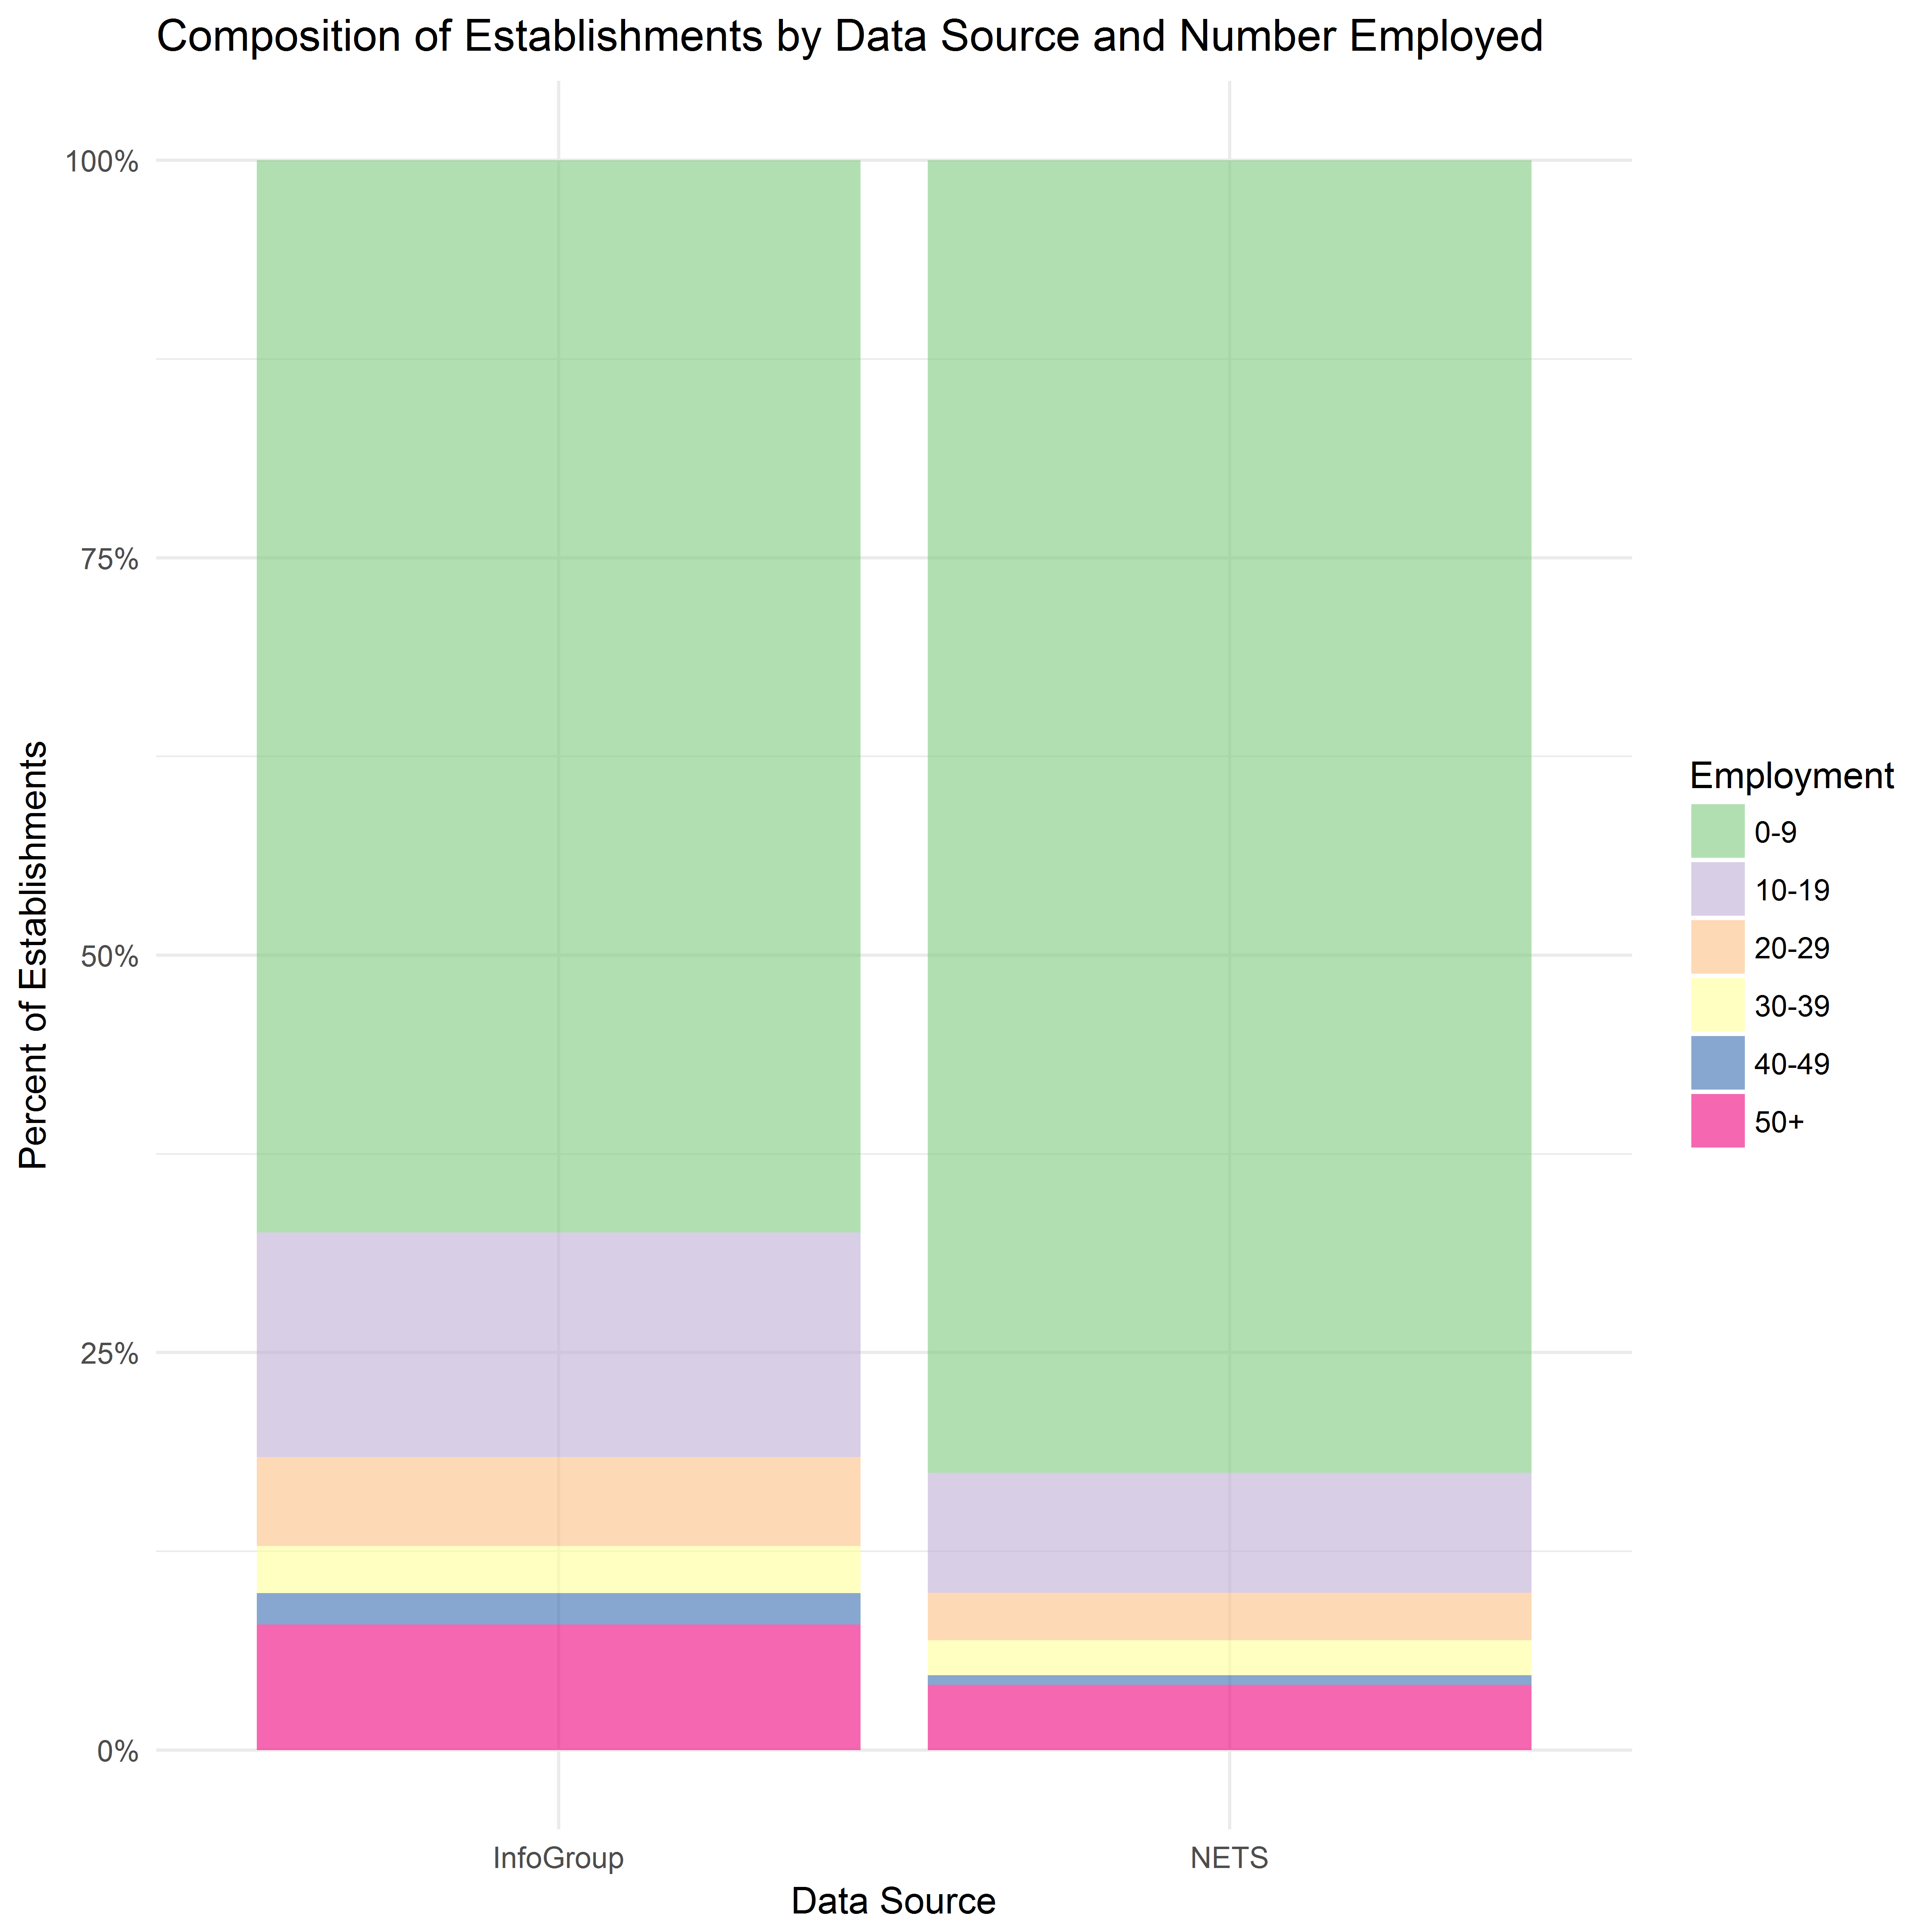
\includegraphics[width = \textwidth]{employmentComposition}
	\caption{Percentage of Establishments at Six Employment Levels.}
\end{figure}
\section{One-to-One Comparison of InfoGroup Sample to NETS Data}
For the random sample of 143 InfoGroup records, we manually matched the InfoGroup firms to their counterparts in the NETS dataset. We found 72 matches in total. Of these, there were:
\begin{itemize}
	\item 44 instances where InfoGroup reported more employees than NETS for the same establishment;
	\item 18 instances where NETS reported more employees than InfoGroup for the same establishment; and
	\item 10 instances where employment was the same in both NETS and InfoGroup.
\end{itemize}
The results indicate that, while InfoGroup has fewer overall records, it tends to report more employees than NETS for identical establishments. The average absolute percentage difference (see Footnote 2) between NETS and InfoGroup employment was 79.32\%, and the median was 66.67\%.
\section{Large Employers}
It is important to compare large employers in Conshohocken for at least three reasons: 1) They are the most visible employers in the area and therefore the easiest to verify; 2) They skew employment totals for a single geographic unit, making it important that they are correctly placed; and 3) Small percentage differences between data sources for these establishments can translate into large aggregate differences in employment for the area. Figure 2, \textit{Distribution of Establishments by Employment and Source}, shows the InfoGroup and NETS records with over 50 employees. Accounting for the overall difference in the number of records between NETS and InfoGroup, NETS reports establishments with roughly 50 employees twice as often as InfoGroup. This may drive the overall difference in employment tallies between NETS and InfoGroup for the study area.\par
\begin{figure}[h]
	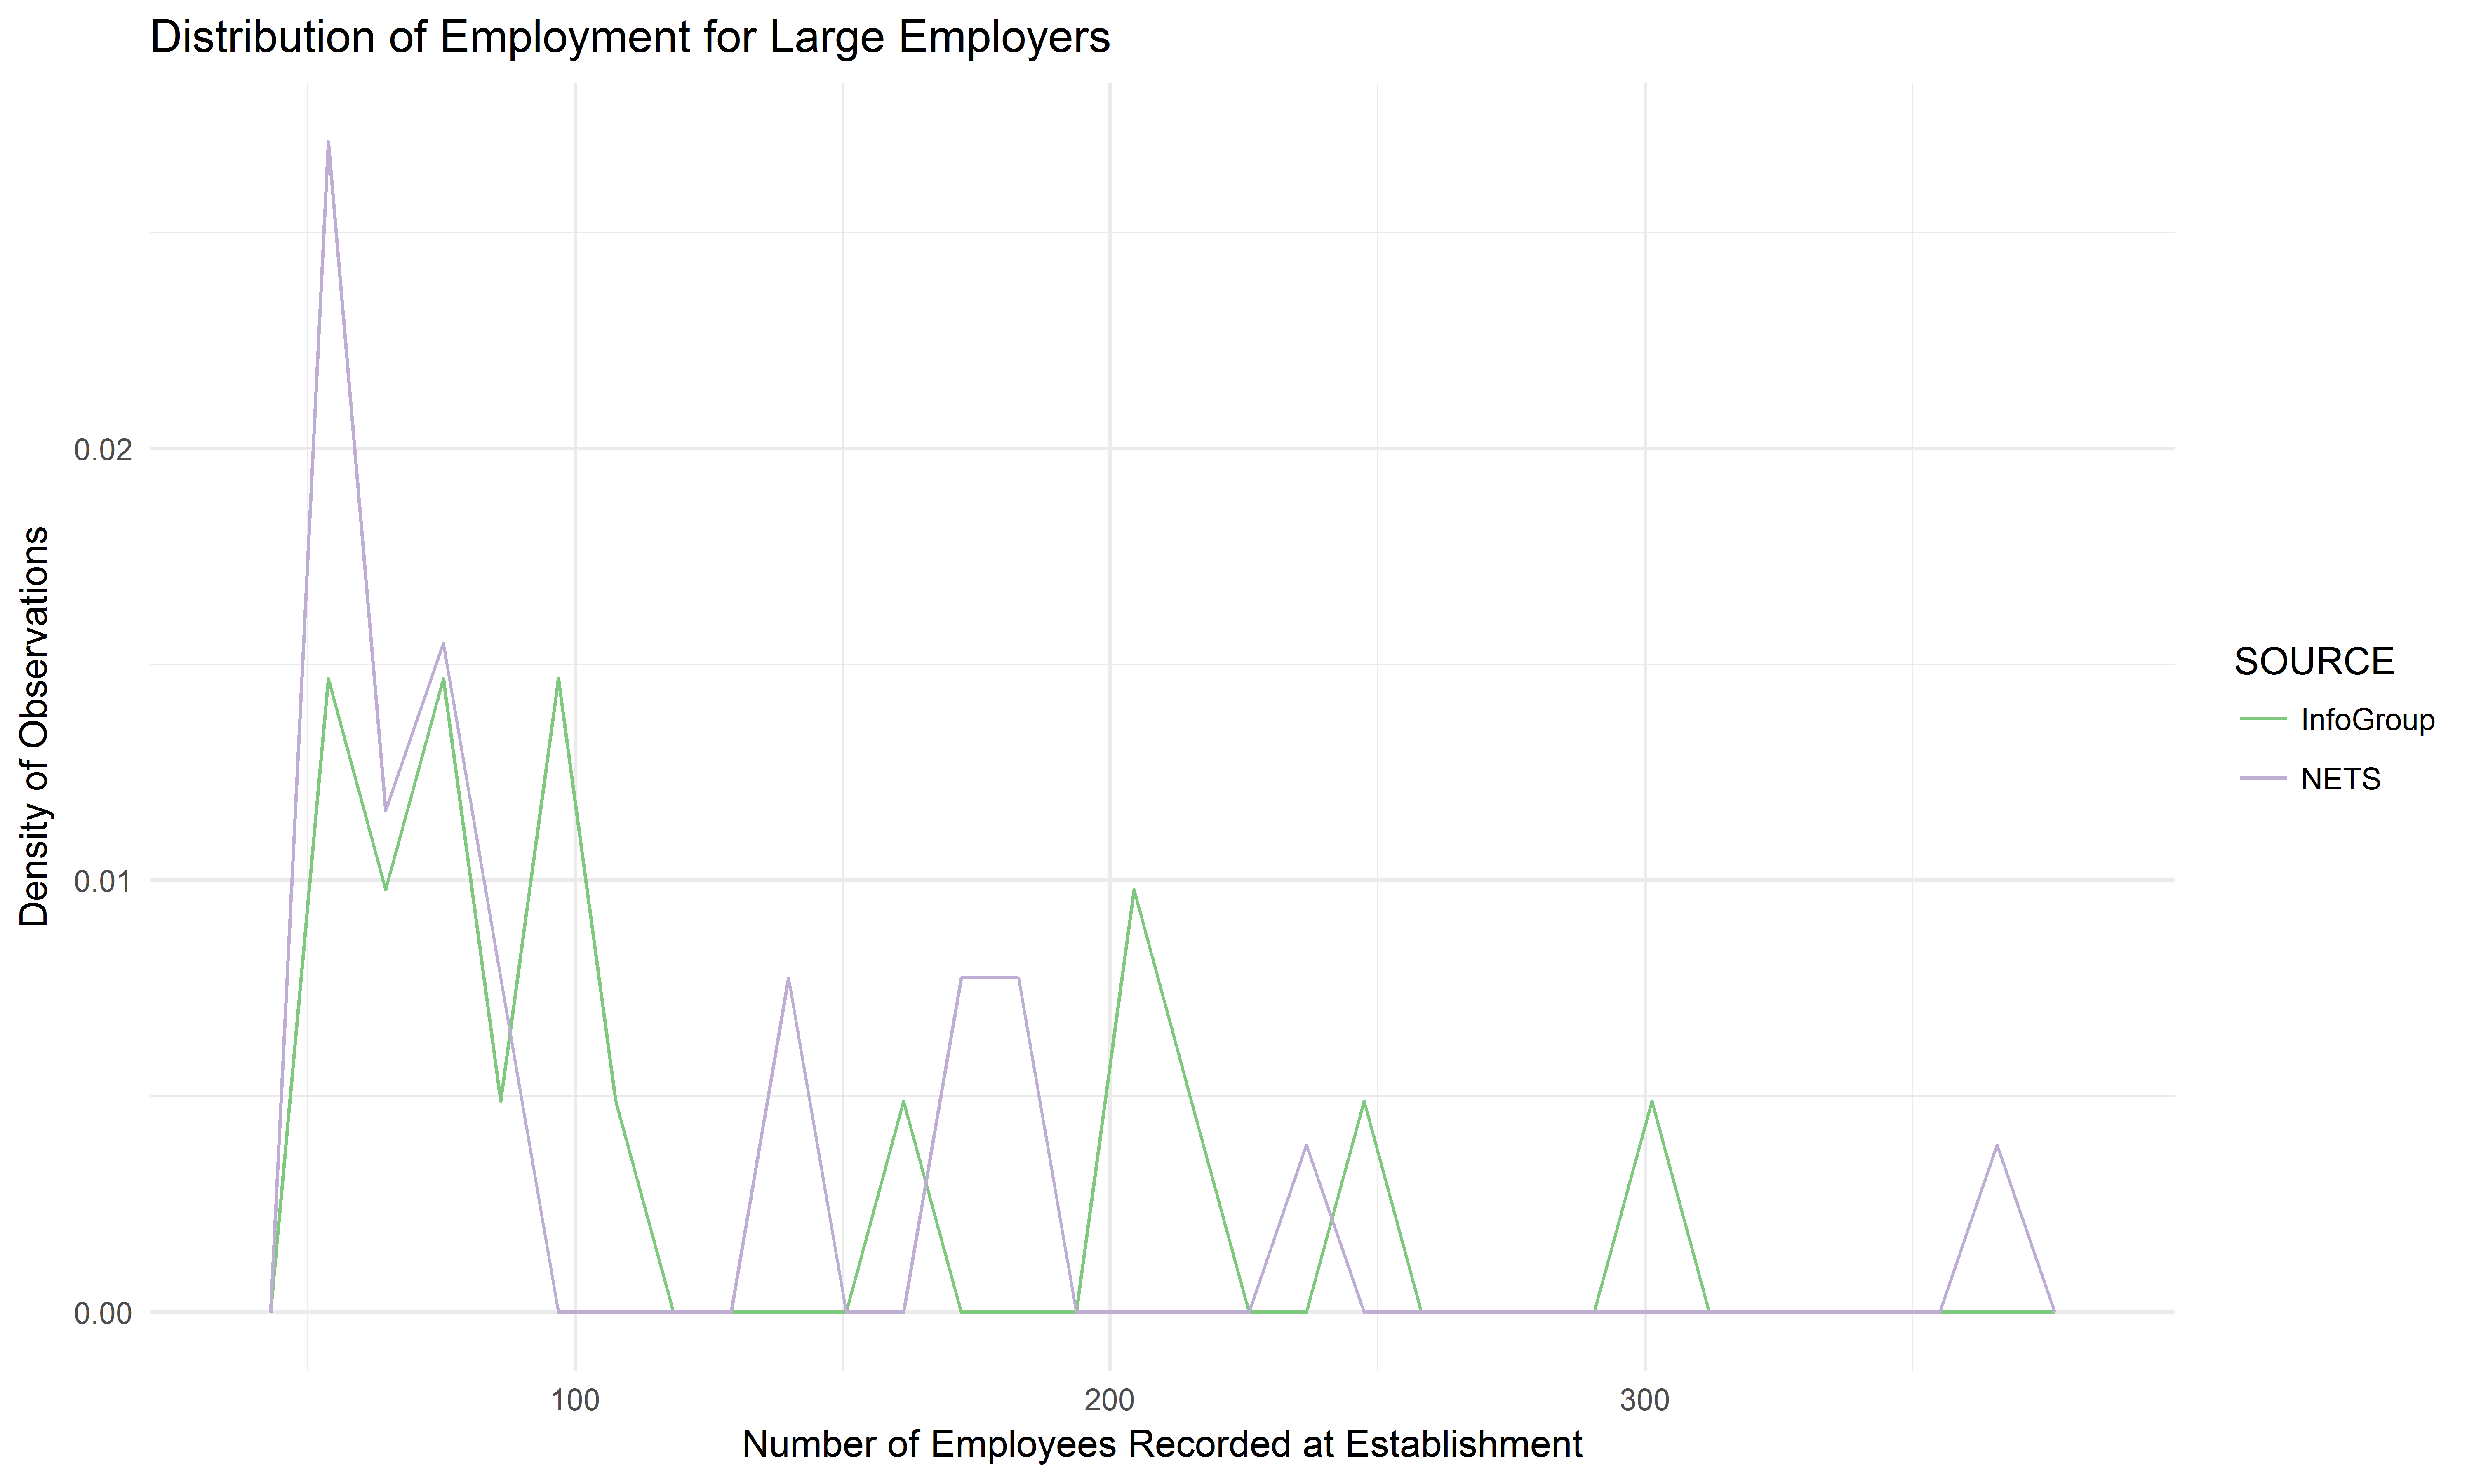
\includegraphics[width = \textwidth]{frequencyLgEmp}
	\caption{Distribution of Establishments by Employment and Source.}
\end{figure}
24 establishments in NETS and 19 in InfoGroup have a total reported number of employees exceeding 50. Of these, 7 large employers are present in both datasets. View Table 5, \textit{Differences in Employment for Seven Large Employers} for employment counts by employer and data source. In four instances, InfoGroup reported more employees than NETS for the same establishment. However, it is worth highlighting two employers: Employer D, where NETS reported 113 more employees than InfoGroup; and Employer E, where InfoGroup reported 118 more employees than NETS. Employer D occupies only one floor of a modest-sized office building: it is likely that the InfoGroup record is closer to the true number of employed in this instance. Furthermore, an online search shows that Employer E self-reports as having over 250 employees at this particular location, pointing again to the InfoGroup record as the more accurate record. Further investigation of the veracity of large employer records might indicate which of these data sources is more reliable in general.
\begin{table}[h]
	\begin{center}
		\begin{tabular}{ r | c c }
			Employer & NETS & InfoGroup \\
			\hline
			\hline
			A & 56 & 75 \\
			\hline 
			B & 56 & 64 \\
			\hline 
			C & 171 & 165 \\
			\hline
			D & 363 & 250 \\
			\hline 
			E & 182 & 300 \\
			\hline 
			F & 138 & 110 \\
			\hline 
			G & 60 & 75 \\
			\hline
		\end{tabular}
	\end{center}
	\caption{Differences in Employment for Seven Large Employers.}
\end{table}
\section{Overall Data Quality}
This section, as with the rest of the analysis, assumes NETS data is already clean and consistent. To evaluate the overall quality of InfoGroup data, we took a sample (\textit{n} = 143) of the InfoGroup data for Conshohocken and manually cleaned it:


\end{document}